\subsection{Data \& Tools}
\label{data-and-tools}
We have identified 4 similar datasets. We have also identified 4 candidate toolsets. We have set time aside to select and augment the data, and to evaluate the tools.

The \textbf{ShapeNet} repository (\cite{chang2015shapenet}) "is an ongoing effort to establish a richly-annotated, large-scale dataset of 3D shapes". Subset data are provided in \textbf{ShapeNetCore}, containing over 50 common object categories and over 50k unique 3D models, and \textbf{ShapeNetSem}, a smaller, more densely annotated set of 12k models and 270 categories, manually verified for labels, consistent alignment, real-world dimensions and estimates of material composition at the category level, as well as estimates of total volume and weight.

The \textbf{ObjectNet3D} repository (\cite{xiang2016objectnet3d}) consists of 100 object categories, 90k 2D
images, 200k objects in these images and 44k 3D shapes. The images
are collected from the ImageNet repository (\cite{imagenet_cvpr09}), while the 3D shapes
are from the ShapeNet repository (\cite{chang2015shapenet}). In addition to 2D bounding box annotations for objects of interest, a key aspect of ObjectNet3D is that each object
in an image is aligned with a 3D shape. The alignment enables
the 3D shape to be projected onto the image, where the projection of the 3D shape matches the
corresponding 2D object in the image (Fig. \ref{fig:ObjectNet3D}). The alignment
between 2D and 3D provides 3D annotations to objects in 2D images, i.e., the
3D pose annotation and the closest 3D shape annotation for a 2D object.  

The \textbf{ScanNet} repository (\cite{dai2017scannet}) is an RGB-D video dataset containing 2.5M views in 1513 scenes annotated with 3D camera poses, surface reconstructions, and semantic segmentations. The annotation process includes placing a closely matching 3D model from a large database in the scene, precisely aligning each model to the 3D position of a corresponding model in the reconstructed indoor scene. ScanNet uses the same categories as ShapeNet and ModelNet (see next).  

\textbf{ModelNet} (\cite{ModelNetwu20143d}) is a large-scale 3D CAD model dataset containing 151,128 3D CAD models, downloaded 3D CAD models from 3D Warehouse, and Yobi3D search engine indexing 261 CAD model websites, belonging to 660 unique object categories. It was built specifically to train the \textit{3D Shapenets} model. 

\begin{figure}[h]
 \centering 
 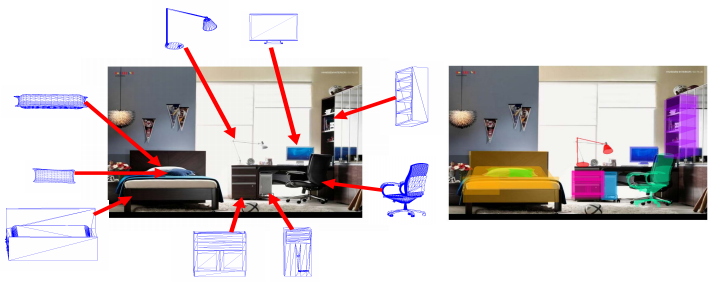
\includegraphics[width=\columnwidth]{figures/ObjectNet3D.png}
 \caption{Example image in the ObjectNet repository with 2D objects aligned with 3D shapes. The alignment enables each 3D shape to be projected onto the image, where its projection
overlaps with the 2D object as shown in the image on the right}
 \label{fig:ObjectNet3D}
\end{figure}  

Time allowing we would like to build a \textbf{synthetic dataset}, though this might prove over-ambitious given our tight schedule - the final dissertation must be delivered by December 21st, 2020.

For prototyping we have identified \textbf{PyTorch}, including the recently (February 2020) released \textbf{PyTorch3D}, \textbf{Keras} (Python TensorFlow wrapper), \textbf{TensorFlow Lite for Microcontrollers} and  \textbf{MATLAB} toolkits as potential tools, all to be used under open source licenses, except MATLAB to be used under an academic license.